\documentclass[letterpaper,12pt]{article}\usepackage[]{graphicx}\usepackage[]{color}
%% maxwidth is the original width if it is less than linewidth
%% otherwise use linewidth (to make sure the graphics do not exceed the margin)
\makeatletter
\def\maxwidth{ %
  \ifdim\Gin@nat@width>\linewidth
    \linewidth
  \else
    \Gin@nat@width
  \fi
}
\makeatother

\definecolor{fgcolor}{rgb}{0.345, 0.345, 0.345}
\newcommand{\hlnum}[1]{\textcolor[rgb]{0.686,0.059,0.569}{#1}}%
\newcommand{\hlstr}[1]{\textcolor[rgb]{0.192,0.494,0.8}{#1}}%
\newcommand{\hlcom}[1]{\textcolor[rgb]{0.678,0.584,0.686}{\textit{#1}}}%
\newcommand{\hlopt}[1]{\textcolor[rgb]{0,0,0}{#1}}%
\newcommand{\hlstd}[1]{\textcolor[rgb]{0.345,0.345,0.345}{#1}}%
\newcommand{\hlkwa}[1]{\textcolor[rgb]{0.161,0.373,0.58}{\textbf{#1}}}%
\newcommand{\hlkwb}[1]{\textcolor[rgb]{0.69,0.353,0.396}{#1}}%
\newcommand{\hlkwc}[1]{\textcolor[rgb]{0.333,0.667,0.333}{#1}}%
\newcommand{\hlkwd}[1]{\textcolor[rgb]{0.737,0.353,0.396}{\textbf{#1}}}%
\let\hlipl\hlkwb

\usepackage{framed}
\makeatletter
\newenvironment{kframe}{%
 \def\at@end@of@kframe{}%
 \ifinner\ifhmode%
  \def\at@end@of@kframe{\end{minipage}}%
  \begin{minipage}{\columnwidth}%
 \fi\fi%
 \def\FrameCommand##1{\hskip\@totalleftmargin \hskip-\fboxsep
 \colorbox{shadecolor}{##1}\hskip-\fboxsep
     % There is no \\@totalrightmargin, so:
     \hskip-\linewidth \hskip-\@totalleftmargin \hskip\columnwidth}%
 \MakeFramed {\advance\hsize-\width
   \@totalleftmargin\z@ \linewidth\hsize
   \@setminipage}}%
 {\par\unskip\endMakeFramed%
 \at@end@of@kframe}
\makeatother

\definecolor{shadecolor}{rgb}{.97, .97, .97}
\definecolor{messagecolor}{rgb}{0, 0, 0}
\definecolor{warningcolor}{rgb}{1, 0, 1}
\definecolor{errorcolor}{rgb}{1, 0, 0}
\newenvironment{knitrout}{}{} % an empty environment to be redefined in TeX

\usepackage{alltt}
\usepackage{amsmath,epsfig,setspace,multirow,url,fancyhdr}
\usepackage{enumitem}
\usepackage{arabtex}
\usepackage{rotating}
% === graphic packages ===
\usepackage{graphicx,textcomp}
% === bibliography package ===
\usepackage{natbib}
% === margin and formatting ===
\usepackage{vmargin}
\setpapersize{USletter}
\topmargin=0in
\usepackage{color}
\usepackage{amssymb}
\usepackage[all]{xy}
\usepackage{lscape}
\usepackage{tikz}
\usetikzlibrary{arrows}
\numberwithin{equation}{section}
% === dcolumn package ===
\usepackage{dcolumn}
\newcolumntype{.}{D{.}{.}{-1}}
\newcolumntype{d}[1]{D{.}{.}{#1}}
% === additional packages ===
\usepackage{color,setspace}
\definecolor{spot}{rgb}{0.6,0,0}
\usepackage{latexsym,bm,subfigure,breqn,pdflscape,float,enumitem,xcolor,booktabs,etex}
\usepackage[hidelinks]{hyperref}
\usepackage{lineno}

\linenumbers

\title{252L - Problem Set 1}
\author{Klint Kanopka}
\date{\today}
\IfFileExists{upquote.sty}{\usepackage{upquote}}{}
\begin{document}
\maketitle



\section{Bernoulli Random Variables}

Q. Compute all the correlations of the columns of this matrix (x1). What do you notice?

\begin{knitrout}
\definecolor{shadecolor}{rgb}{0.969, 0.969, 0.969}\color{fgcolor}\begin{kframe}
\begin{alltt}
\hlkwd{set.seed}\hlstd{(}\hlnum{12311}\hlstd{)}
\hlstd{x1}\hlkwb{<-}\hlkwd{matrix}\hlstd{(}\hlkwd{rbinom}\hlstd{(}\hlnum{1000}\hlstd{,}\hlnum{1}\hlstd{,}\hlnum{.5}\hlstd{),}\hlnum{100}\hlstd{,}\hlnum{10}\hlstd{)}

\hlkwd{cor}\hlstd{(x1)}
\end{alltt}
\begin{verbatim}
##               [,1]         [,2]         [,3]          [,4]         [,5]
##  [1,]  1.000000000  0.008410789 -0.009896948 -0.3032770731  0.094629567
##  [2,]  0.008410789  1.000000000  0.089886562 -0.0669602615 -0.057570773
##  [3,] -0.009896948  0.089886562  1.000000000  0.0295469723 -0.125809070
##  [4,] -0.303277073 -0.066960261  0.029546972  1.0000000000  0.089214650
##  [5,]  0.094629567 -0.057570773 -0.125809070  0.0892146505  1.000000000
##  [6,]  0.237526763  0.130744090 -0.001602564 -0.0525279507  0.035484609
##  [7,]  0.081814407 -0.074443750  0.047043222 -0.0988646639  0.060409150
##  [8,]  0.098085811 -0.016333199  0.059259270  0.0455242322 -0.103165975
##  [9,] -0.149960697 -0.107907043  0.053719716 -0.0004168548 -0.001638407
## [10,]  0.025551766  0.179665184  0.060860872  0.0365014114 -0.058030861
##               [,6]         [,7]        [,8]          [,9]       [,10]
##  [1,]  0.237526763  0.081814407  0.09808581 -0.1499606967  0.02555177
##  [2,]  0.130744090 -0.074443750 -0.01633320 -0.1079070433  0.17966518
##  [3,] -0.001602564  0.047043222  0.05925927  0.0537197158  0.06086087
##  [4,] -0.052527951 -0.098864664  0.04552423 -0.0004168548  0.03650141
##  [5,]  0.035484609  0.060409150 -0.10316597 -0.0016384067 -0.05803086
##  [6,]  1.000000000  0.087597723  0.09929932 -0.1904608106 -0.05925927
##  [7,]  0.087597723  1.000000000  0.02350749  0.0090628774  0.05755282
##  [8,]  0.099299317  0.023507488  1.00000000  0.0370118105  0.08043217
##  [9,] -0.190460811  0.009062877  0.03701181  1.0000000000  0.08500515
## [10,] -0.059259270  0.057552816  0.08043217  0.0850051472  1.00000000
\end{verbatim}
\end{kframe}
\end{knitrout}

The correlation matrix has 1's along the diagonal, which makes sense because: 
			\[ \sigma(x,x)=1 \]
The matrix is also symmetric about the diagonal, which makes sense because:
			\[ \sigma(x,y) = \sigma(y,x) \]  
The correlations are also relatively small, which makes sense because the data is generated randomly.


Q. Compute the row sums. What is the variation in row sums?

\begin{knitrout}
\definecolor{shadecolor}{rgb}{0.969, 0.969, 0.969}\color{fgcolor}\begin{kframe}
\begin{alltt}
\hlkwd{var}\hlstd{(}\hlkwd{rowSums}\hlstd{(x1))}
\end{alltt}
\begin{verbatim}
## [1] 2.706667
\end{verbatim}
\end{kframe}
\end{knitrout}

The variance of the row sums is $2.706667$.  Given the context of the following question, this represents variance in total test scores across individuals.


Q. If you considered the 1s/0s correct and incorrect responses to test items (where the rows are people and the columns are items), does this seem like it could have come from a realistic scenario?



Probably not, because the correlations are so small.  One might also expect a test to have "easy" and "hard" questions, which this randomly constructed matrix does not indicate when looking at the column sums.


Q. Now go back through the above questions and see what you make of this new matrix x2. Specifically, how does it compare to the first matrix x1 in terms of whether it seems like a realistic set of item responses? What characteristics (feel free to explore other features of the data) influence your opinion on this point?

\begin{knitrout}
\definecolor{shadecolor}{rgb}{0.969, 0.969, 0.969}\color{fgcolor}\begin{kframe}
\begin{alltt}
\hlkwd{var}\hlstd{(}\hlkwd{rowSums}\hlstd{(x2))}
\end{alltt}
\begin{verbatim}
## [1] 5.111111
\end{verbatim}
\end{kframe}
\end{knitrout}

For $x_2$, the matrix still has 1's along the diagonal and is symmetric about the diagonal, but generally speaking the correlations are higher than they were in $x_1$.

The variance of the row sums is $5.111111$.  The variation in row sums here is higher.  If you look at histograms of the row sums, the data is also somewhat more uniformly distributed in $x_2$ than in $x_1$, so it makes sense that the variance would be higher in this situation.

\begin{knitrout}
\definecolor{shadecolor}{rgb}{0.969, 0.969, 0.969}\color{fgcolor}
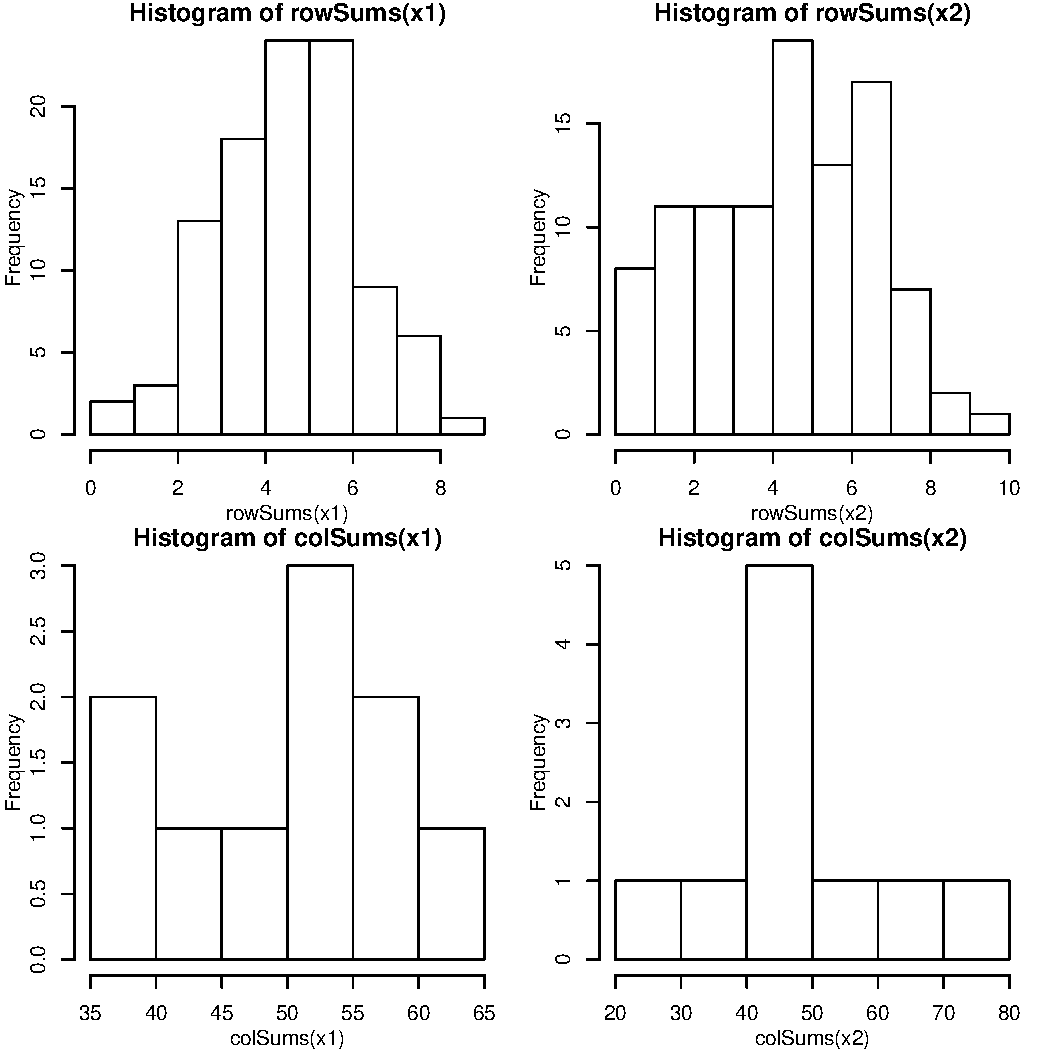
\includegraphics[width=\maxwidth]{figure/unnamed-chunk-6-1} 

\end{knitrout}


Looking at histograms of row and column sums in $x_1$ and $x_2$, $x_2$ is less clearly normally distributed, meaning that there are respondents at lower ability levels, but a sharper drop off after 7 (and 8) correct.  More than anything, the difference in the variance between the column sums (61.7 in $x_1$ and 242.7 in $x_2$) implies that all the items in $x_1$ would have been of similar difficulty, whereas the items in $x_2$ are of varying difficulty.  If you look at the histogram of column sums, however, you will see that this is blatantly untrue.  The histogram of column sums for $x_2$, specifically, is the most damning piece of evidence in favor of $x_1$ being the "real test."

\pagebreak
\section{Logistic Regression}

(1) How would you compare the association between y1/y2 \& x? (2) How would you interpret the regression coefficients from (say) m1? (3) Do m1 and m2 show equivalent model fit? Can you notice anything peculiar about either y1 or y2 (in terms of their association with x)?

\begin{knitrout}
\definecolor{shadecolor}{rgb}{0.969, 0.969, 0.969}\color{fgcolor}\begin{kframe}
\begin{alltt}
\hlkwd{load}\hlstd{(}\hlstr{"ps1-logreg.Rdata"}\hlstd{)}

\hlstd{m1} \hlkwb{<-} \hlkwd{glm}\hlstd{(y1}\hlopt{~}\hlstd{x,df,}\hlkwc{family}\hlstd{=}\hlstr{"binomial"}\hlstd{)}
\hlkwd{plot}\hlstd{(df}\hlopt{$}\hlstd{x,df}\hlopt{$}\hlstd{y1)}
\hlkwd{curve}\hlstd{(}\hlkwd{predict}\hlstd{(m1,}\hlkwd{data.frame}\hlstd{(}\hlkwc{x}\hlstd{=x),}\hlkwc{type}\hlstd{=}\hlstr{"resp"}\hlstd{),}\hlkwc{add}\hlstd{=}\hlnum{TRUE}\hlstd{)}
\end{alltt}
\end{kframe}
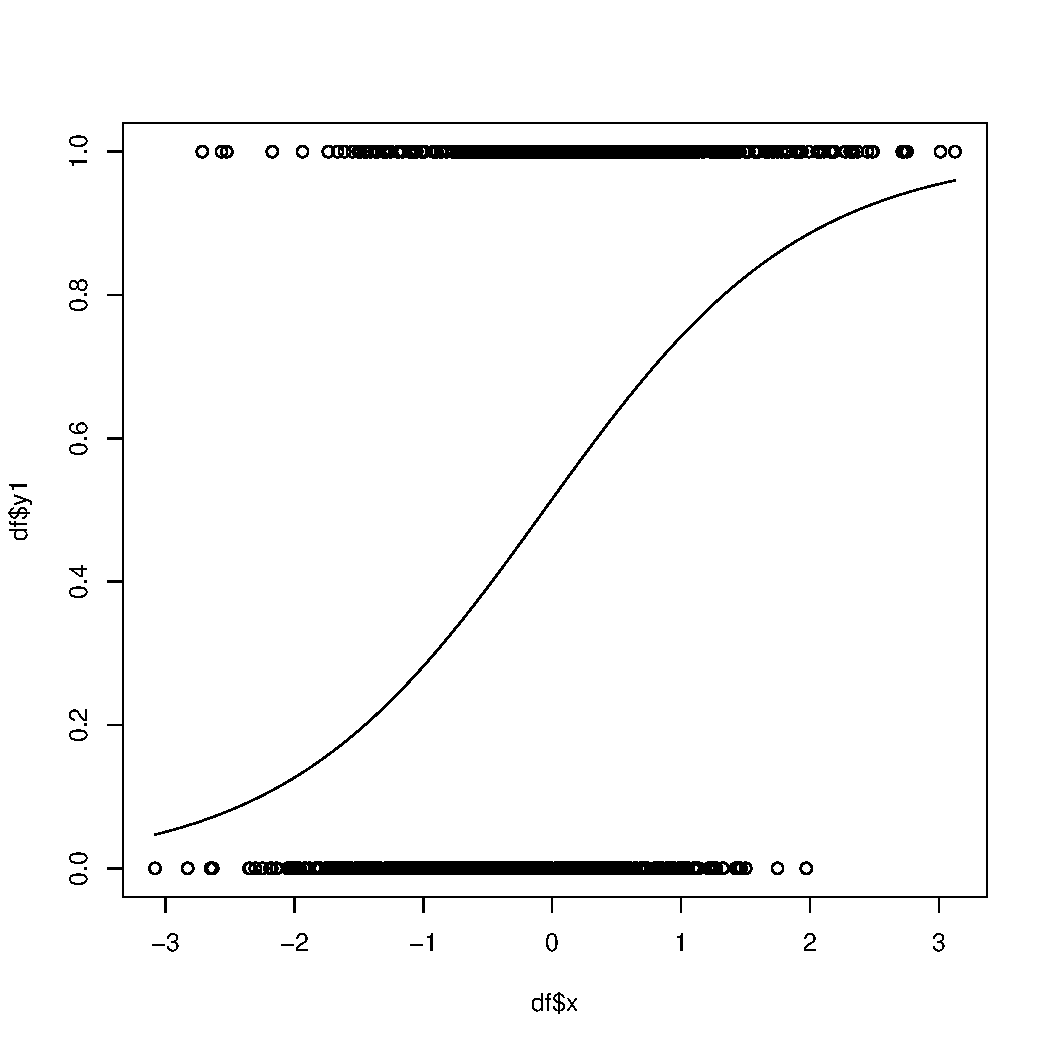
\includegraphics[width=\maxwidth]{figure/unnamed-chunk-7-1} 
\begin{kframe}\begin{alltt}
\hlstd{m2} \hlkwb{<-} \hlkwd{glm}\hlstd{(y2}\hlopt{~}\hlstd{x,df,}\hlkwc{family}\hlstd{=}\hlstr{"binomial"}\hlstd{)}
\hlkwd{plot}\hlstd{(df}\hlopt{$}\hlstd{x,df}\hlopt{$}\hlstd{y2)}
\hlkwd{curve}\hlstd{(}\hlkwd{predict}\hlstd{(m2,}\hlkwd{data.frame}\hlstd{(}\hlkwc{x}\hlstd{=x),}\hlkwc{type}\hlstd{=}\hlstr{"resp"}\hlstd{),}\hlkwc{add}\hlstd{=}\hlnum{TRUE}\hlstd{)}
\end{alltt}
\end{kframe}
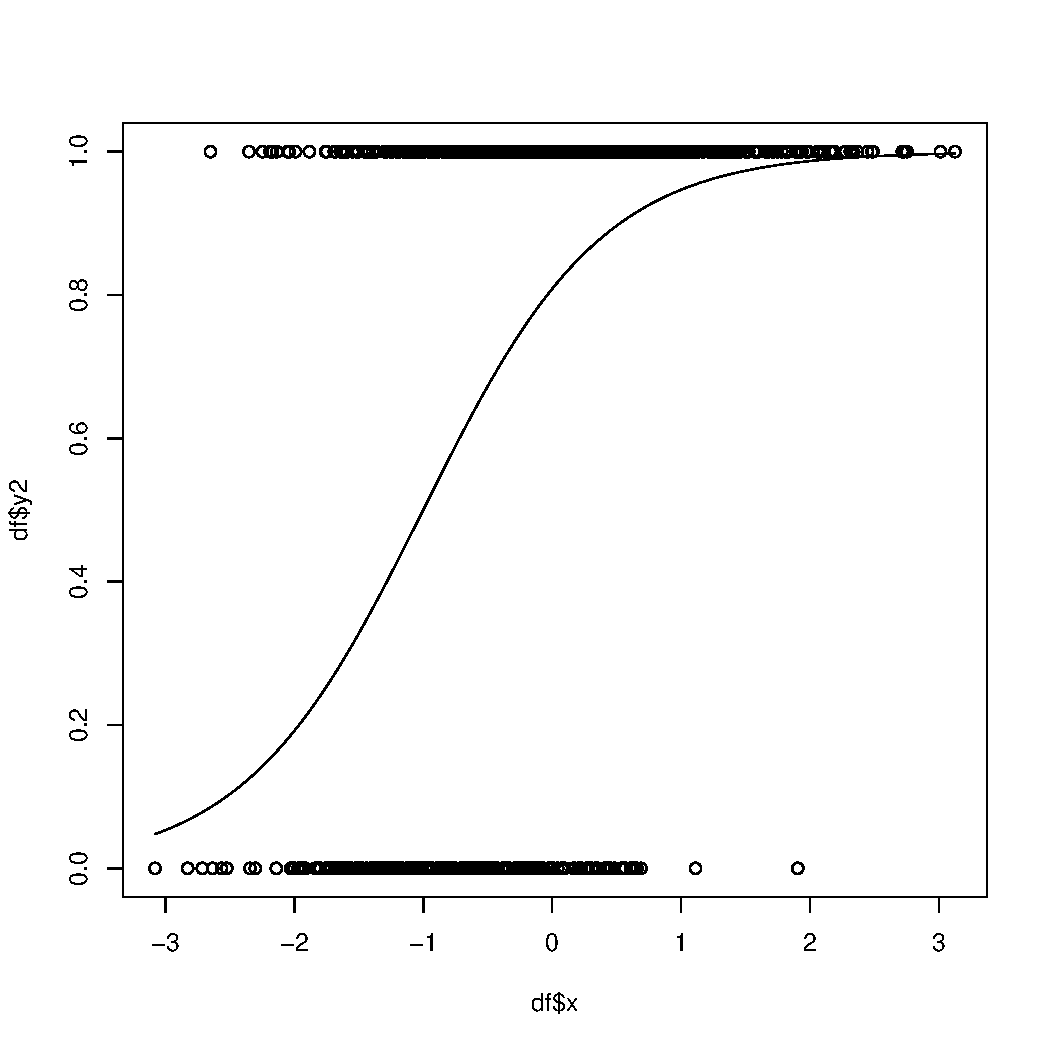
\includegraphics[width=\maxwidth]{figure/unnamed-chunk-7-2} 

\end{knitrout}


	\begin{enumerate}
		\item The association between $x$ and $y_2$ is stronger than the association between x and $y_1$. This is because the AIC, null deviance and residual deviance are lower for $y_2$. In addition, when looking at plots, there is less overlap between the top and bottom sections in the plots of $y_2$ than in $y_1$. In $y_2$, the logistic curve has a steeper transition from minimum value to maximum value.
        
		\item The regression coefficients, $\beta_0$ and $\beta_1$, are related to the shape of the logistic fit. Specifically, $\beta_0$ is related to the intercept. $\beta_1$ is a measure of test item discrimination. $\beta_1$ is related to the slope at the point of inflection, so a higher slope would indicate higher levels of discrimination. $\beta_0$ is related to difficulty, with a lower $\beta_0$ indicating an easier test item. $\beta_0$ is the odds of getting an answer correct when $x = 0$.



\begin{table}[!htbp] \centering 
  \caption{} 
  \label{} 
\begin{tabular}{@{\extracolsep{5pt}}lcc} 
\\[-1.8ex]\hline 
\hline \\[-1.8ex] 
 & \multicolumn{2}{c}{\textit{Dependent variable:}} \\ 
\cline{2-3} 
\\[-1.8ex] & y1 & y2 \\ 
\\[-1.8ex] & (1) & (2)\\ 
\hline \\[-1.8ex] 
 x & 0.996$^{***}$ & 1.440$^{***}$ \\ 
  & (0.084) & (0.109) \\ 
  & & \\ 
 Constant & 0.061 & 1.441$^{***}$ \\ 
  & (0.069) & (0.097) \\ 
  & & \\ 
\hline \\[-1.8ex] 
Observations & 1,000 & 1,000 \\ 
Log Likelihood & $-$602.437 & $-$448.444 \\ 
Akaike Inf. Crit. & 1,208.875 & 900.889 \\ 
\hline 
\hline \\[-1.8ex] 
\textit{Note:}  & \multicolumn{2}{r}{$^{*}$p$<$0.1; $^{**}$p$<$0.05; $^{***}$p$<$0.01} \\ 
\end{tabular} 
\end{table} 



\item From the graphs above, $m_2$ appears to be a better model fit.  One peculiar thing appears to be the enormous level of overlap between the two conditions predicted by $x$ in $y_1$.

	\end{enumerate}







\pagebreak
\section{Likelihood Exploration}
Looks vaguely normalish, no? 

\begin{knitrout}
\definecolor{shadecolor}{rgb}{0.969, 0.969, 0.969}\color{fgcolor}
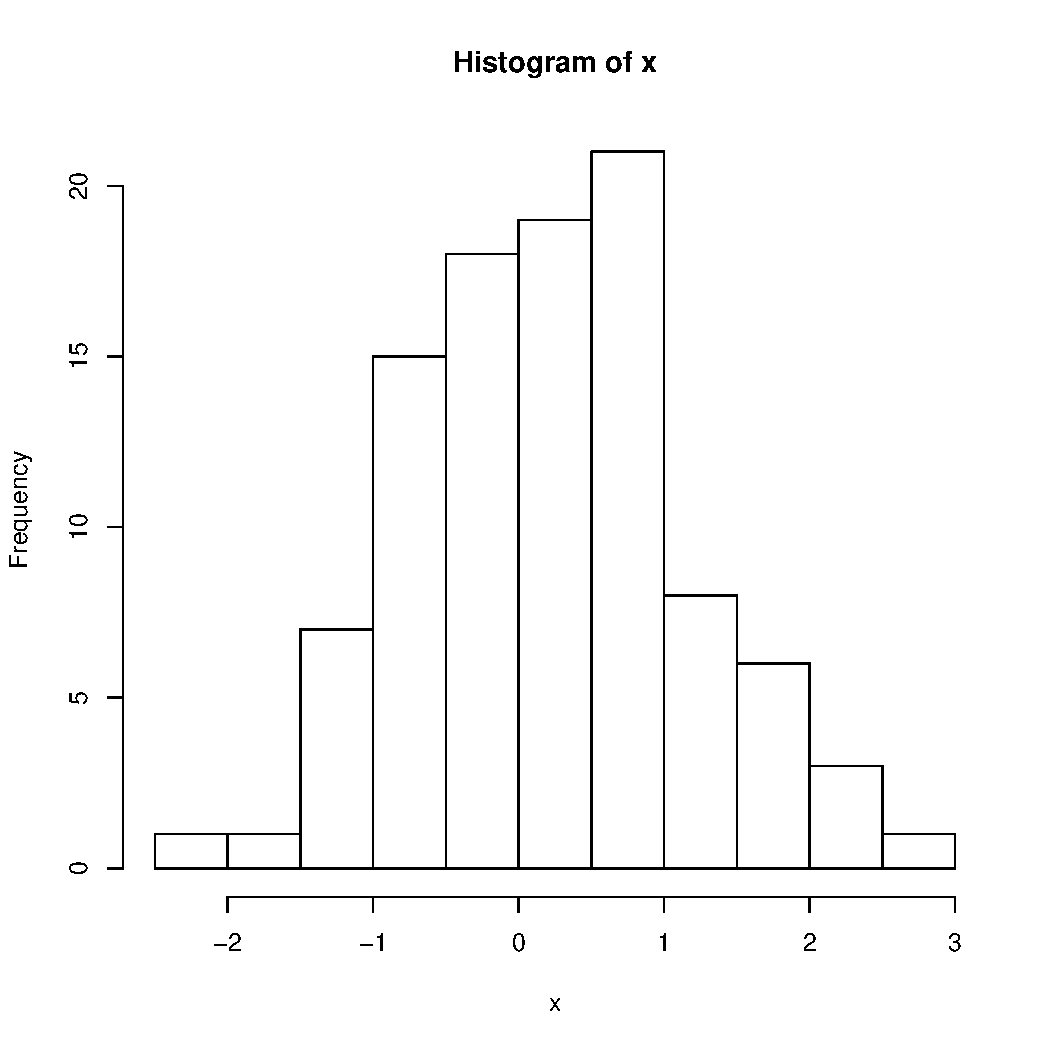
\includegraphics[width=\maxwidth]{figure/unnamed-chunk-9-1} 

\end{knitrout}

Yes, it does.


\begin{knitrout}
\definecolor{shadecolor}{rgb}{0.969, 0.969, 0.969}\color{fgcolor}\begin{kframe}
\begin{alltt}
\hlstd{likelihood}\hlkwb{<-}\hlkwa{function}\hlstd{(}\hlkwc{pars}\hlstd{,}\hlkwc{x}\hlstd{) \{}
    \hlstd{tmp}\hlkwb{<-}\hlkwd{exp}\hlstd{(}\hlopt{-}\hlstd{(x}\hlopt{-}\hlstd{pars[}\hlnum{1}\hlstd{])}\hlopt{^}\hlnum{2}\hlopt{/}\hlstd{(}\hlnum{2}\hlopt{*}\hlstd{pars[}\hlnum{2}\hlstd{]))}
    \hlstd{tmp}\hlopt{/}\hlkwd{sqrt}\hlstd{(}\hlnum{2}\hlopt{*}\hlstd{pars[}\hlnum{2}\hlstd{]}\hlopt{*}\hlstd{pi)}
\hlstd{\}}
\end{alltt}
\end{kframe}
\end{knitrout}

Let's think about what we get if the mean is unknown and the SD=1
Q. what do you notice? 

\begin{knitrout}
\definecolor{shadecolor}{rgb}{0.969, 0.969, 0.969}\color{fgcolor}\begin{kframe}
\begin{alltt}
\hlstd{out}\hlkwb{<-}\hlkwd{list}\hlstd{()}
\hlkwa{for} \hlstd{(m} \hlkwa{in} \hlkwd{seq}\hlstd{(}\hlopt{-}\hlnum{1}\hlstd{,}\hlnum{1}\hlstd{,}\hlkwc{length.out}\hlstd{=}\hlnum{100}\hlstd{)) \{}
    \hlstd{like}\hlkwb{<-}\hlkwd{rep}\hlstd{(}\hlnum{NA}\hlstd{,}\hlkwd{length}\hlstd{(x))}
    \hlkwa{for} \hlstd{(i} \hlkwa{in} \hlnum{1}\hlopt{:}\hlkwd{length}\hlstd{(x)) \{}
        \hlstd{like[i]}\hlkwb{<-}\hlkwd{likelihood}\hlstd{(}\hlkwd{c}\hlstd{(m,}\hlnum{1}\hlstd{),x[i])}
    \hlstd{\}}
    \hlkwd{c}\hlstd{(}\hlkwd{c}\hlstd{(m,}\hlkwd{prod}\hlstd{(like)))}\hlkwb{->}\hlstd{out[[}\hlkwd{as.character}\hlstd{(m) ]]}
\hlstd{\}}
\hlkwd{plot}\hlstd{(}\hlkwd{do.call}\hlstd{(}\hlstr{"rbind"}\hlstd{,out),}\hlkwc{type}\hlstd{=}\hlstr{"b"}\hlstd{)}
\end{alltt}
\end{kframe}
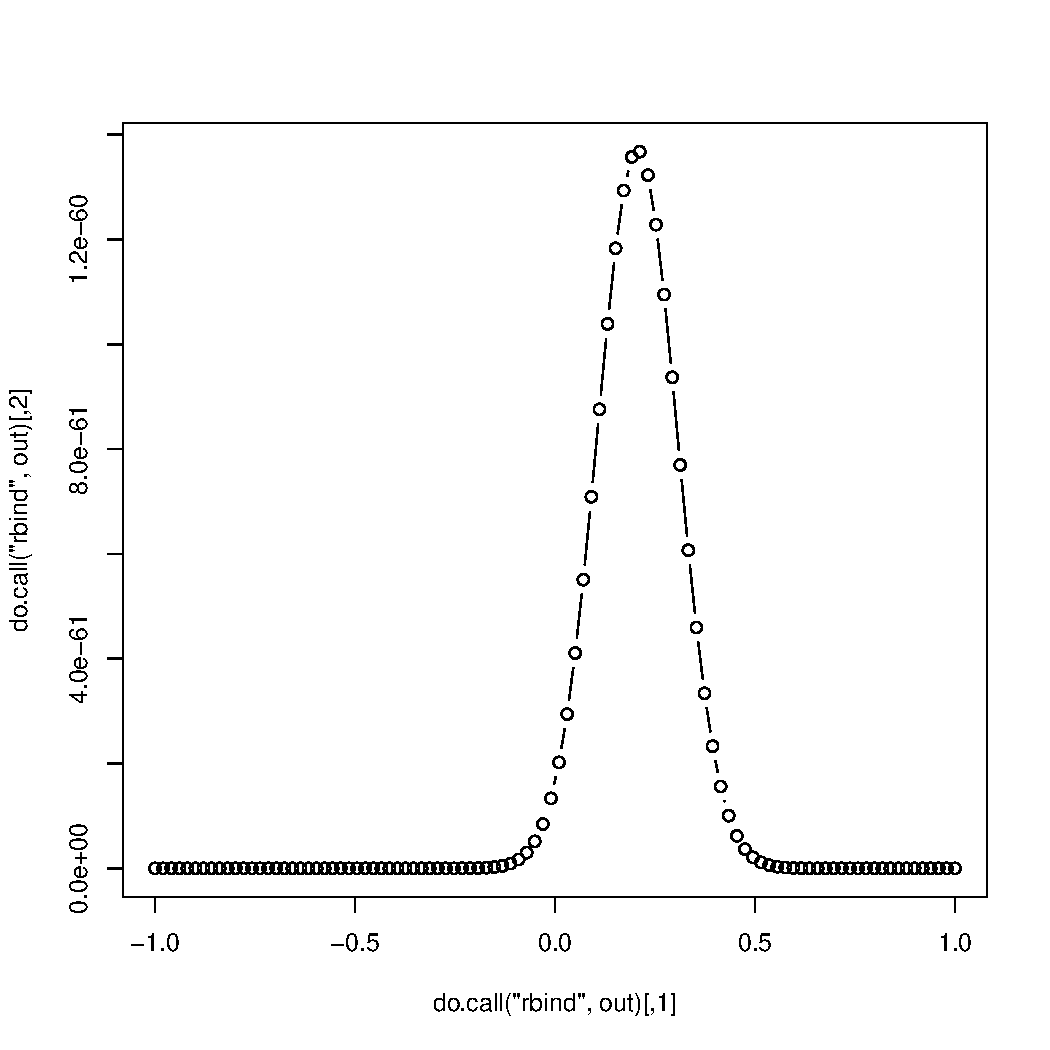
\includegraphics[width=\maxwidth]{figure/unnamed-chunk-11-1} 

\end{knitrout}

The slice of the likelihood surface shown here has a maximum value at our best estimate of the mean.  It's also worth noting that the values for likelihood are really tiny, which is a good reason to use log-likelihood in computational applications.


Q. How do our estimates vary in accuracy as a function of the sample size (change 100 to something much bigger and much smaller in the top line)

\begin{knitrout}
\definecolor{shadecolor}{rgb}{0.969, 0.969, 0.969}\color{fgcolor}\begin{kframe}
\begin{alltt}
\hlstd{ll}\hlkwb{<-}\hlkwa{function}\hlstd{(}\hlkwc{pars}\hlstd{,}\hlkwc{x}\hlstd{) \{}
    \hlstd{likelihood}\hlkwb{<-}\hlkwa{function}\hlstd{(}\hlkwc{pars}\hlstd{,}\hlkwc{x}\hlstd{) \{}
        \hlstd{tmp}\hlkwb{<-}\hlkwd{exp}\hlstd{(}\hlopt{-}\hlstd{(x}\hlopt{-}\hlstd{pars[}\hlnum{1}\hlstd{])}\hlopt{^}\hlnum{2}\hlopt{/}\hlstd{(}\hlnum{2}\hlopt{*}\hlstd{pars[}\hlnum{2}\hlstd{]))}
        \hlstd{tmp}\hlopt{/}\hlkwd{sqrt}\hlstd{(}\hlnum{2}\hlopt{*}\hlstd{pars[}\hlnum{2}\hlstd{]}\hlopt{*}\hlstd{pi)}
    \hlstd{\}}
    \hlstd{like}\hlkwb{<-}\hlkwd{rep}\hlstd{(}\hlnum{NA}\hlstd{,}\hlkwd{length}\hlstd{(x))}
    \hlkwa{for} \hlstd{(i} \hlkwa{in} \hlnum{1}\hlopt{:}\hlkwd{length}\hlstd{(x)) \{}
        \hlstd{like[i]}\hlkwb{<-}\hlkwd{likelihood}\hlstd{(pars,x[i])}
    \hlstd{\}}
    \hlopt{-}\hlnum{1}\hlopt{*}\hlkwd{sum}\hlstd{(}\hlkwd{log}\hlstd{(like))}
\hlstd{\}}
\hlcom{#these are the mean and variance estimates produced by MLE.}
\hlkwd{optim}\hlstd{(}\hlkwc{par}\hlstd{=}\hlkwd{c}\hlstd{(}\hlopt{-}\hlnum{2}\hlstd{,}\hlnum{2}\hlstd{),ll,}\hlkwc{x}\hlstd{=x)}\hlopt{$}\hlstd{par}
\end{alltt}
\begin{verbatim}
## [1] 0.2058405 0.9189130
\end{verbatim}
\end{kframe}
\end{knitrout}

    As the sample size increases, the mean approaches zero and the variance approaches one.
    
    \begin{tabular}{|l|l|l|}
	\hline
	Sample Size & Mean & Variance \\
	\hline
	10 & 0.2335989 & 1.3643526 \\
	100 & 0.1675501 & 0.9539125 \\
	1000 & -0.02798667 & 0.95039213 \\
	10000 & 0.0014444 & 1.0368603 \\
	\hline
	\end{tabular}

\pagebreak
\section{Item Quality}

Consider the item statistics (p-values \& item-total correlations) discussed in the Crocker \& Algina text. What do you think? As a point of contrast, consider them vis-a-vis the item statistics generated by this data:

\begin{knitrout}
\definecolor{shadecolor}{rgb}{0.969, 0.969, 0.969}\color{fgcolor}\begin{kframe}
\begin{alltt}
\hlstd{out}\hlkwb{<-}\hlkwd{list}\hlstd{()}

\hlcom{##CTT item analysis}
\hlcom{##this function will compute CTT item statistics}
\hlstd{item_analysis}\hlkwb{<-}\hlkwa{function}\hlstd{(}\hlkwc{resp}\hlstd{) \{}
    \hlstd{pv}\hlkwb{<-}\hlkwd{colMeans}\hlstd{(resp,}\hlkwc{na.rm}\hlstd{=}\hlnum{TRUE}\hlstd{)}
    \hlstd{r.xt}\hlkwb{<-}\hlkwd{numeric}\hlstd{()}
    \hlkwd{rowSums}\hlstd{(resp,}\hlkwc{na.rm}\hlstd{=}\hlnum{TRUE}\hlstd{)}\hlkwb{->}\hlstd{ss}
    \hlkwa{for} \hlstd{(i} \hlkwa{in} \hlnum{1}\hlopt{:}\hlkwd{ncol}\hlstd{(resp)) \{}
        \hlkwd{cor}\hlstd{(ss,resp[,i],}\hlkwc{use}\hlstd{=}\hlstr{'p'}\hlstd{)}\hlkwb{->}\hlstd{r.xt[i]}
    \hlstd{\}}
    \hlcom{#return matrix of the p-values and the item/total correlations}
    \hlkwd{cbind}\hlstd{(pv,r.xt)}
\hlstd{\}}

\hlstd{resp1} \hlkwb{<-}\hlkwd{read.table}\hlstd{(}\hlstr{"emp-rasch.txt"}\hlstd{,}\hlkwc{header}\hlstd{=}\hlnum{FALSE}\hlstd{)}
\hlstd{out[[}\hlnum{1}\hlstd{]]}\hlkwb{<-}\hlkwd{item_analysis}\hlstd{(resp1)}

\hlstd{resp2} \hlkwb{<-}\hlkwd{read.table}\hlstd{(}\hlstr{"rasch.txt"}\hlstd{,}\hlkwc{header}\hlstd{=}\hlnum{FALSE}\hlstd{)}
\hlstd{out[[}\hlnum{2}\hlstd{]]}\hlkwb{<-}\hlkwd{item_analysis}\hlstd{(resp2)}

\hlkwd{par}\hlstd{(}\hlkwc{mfrow}\hlstd{=}\hlkwd{c}\hlstd{(}\hlnum{2}\hlstd{,}\hlnum{1}\hlstd{),}\hlkwc{mgp}\hlstd{=}\hlkwd{c}\hlstd{(}\hlnum{2}\hlstd{,}\hlnum{1}\hlstd{,}\hlnum{0}\hlstd{),}\hlkwc{mar}\hlstd{=}\hlkwd{c}\hlstd{(}\hlnum{3}\hlstd{,}\hlnum{3}\hlstd{,}\hlnum{1}\hlstd{,}\hlnum{1}\hlstd{))}

\hlkwd{plot}\hlstd{(out[[}\hlnum{1}\hlstd{]])}
\hlkwd{plot}\hlstd{(out[[}\hlnum{2}\hlstd{]])}
\end{alltt}
\end{kframe}
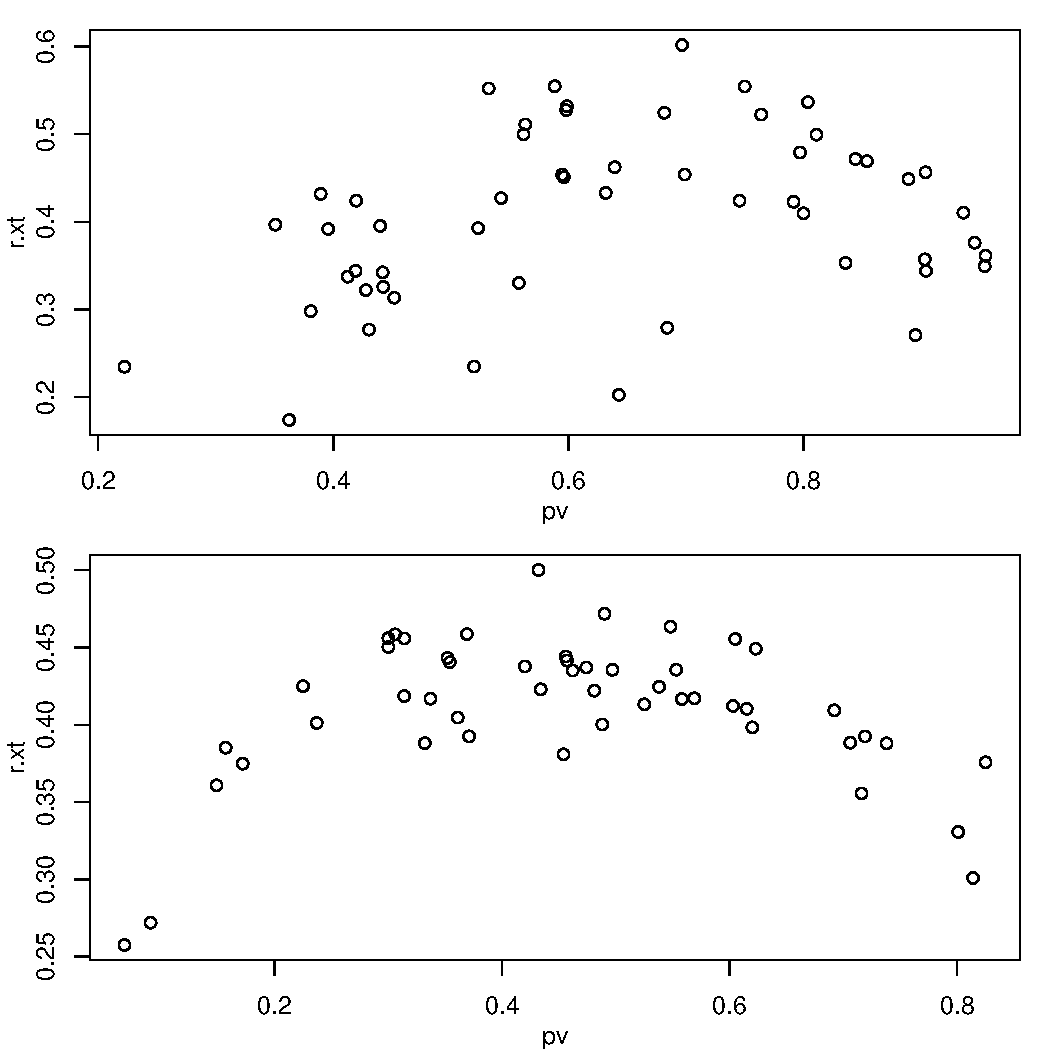
\includegraphics[width=\maxwidth]{figure/unnamed-chunk-13-1} 
\begin{kframe}\begin{alltt}
\hlkwd{par}\hlstd{(}\hlkwc{mfrow}\hlstd{=}\hlkwd{c}\hlstd{(}\hlnum{2}\hlstd{,}\hlnum{2}\hlstd{),}\hlkwc{mgp}\hlstd{=}\hlkwd{c}\hlstd{(}\hlnum{2}\hlstd{,}\hlnum{1}\hlstd{,}\hlnum{0}\hlstd{),}\hlkwc{mar}\hlstd{=}\hlkwd{c}\hlstd{(}\hlnum{3}\hlstd{,}\hlnum{3}\hlstd{,}\hlnum{1}\hlstd{,}\hlnum{1}\hlstd{))}
\hlstd{pf}\hlkwb{<-}\hlkwa{function}\hlstd{(}\hlkwc{x}\hlstd{) \{}
    \hlkwd{plot}\hlstd{(}\hlkwd{density}\hlstd{(x[,}\hlnum{1}\hlstd{]),}\hlkwc{xlim}\hlstd{=}\hlkwd{c}\hlstd{(}\hlnum{0}\hlstd{,}\hlnum{1}\hlstd{),}\hlkwc{xlab}\hlstd{=}\hlstr{"density, p-values"}\hlstd{)}
    \hlkwd{plot}\hlstd{(}\hlkwd{density}\hlstd{(x[,}\hlnum{2}\hlstd{]),}\hlkwc{xlim}\hlstd{=}\hlkwd{c}\hlstd{(}\hlnum{0}\hlstd{,}\hlnum{1}\hlstd{),}\hlkwc{xlab}\hlstd{=}\hlstr{"density, item-total correlations"}\hlstd{)}
\hlstd{\}}
\hlkwd{lapply}\hlstd{(out,pf)}
\end{alltt}
\end{kframe}
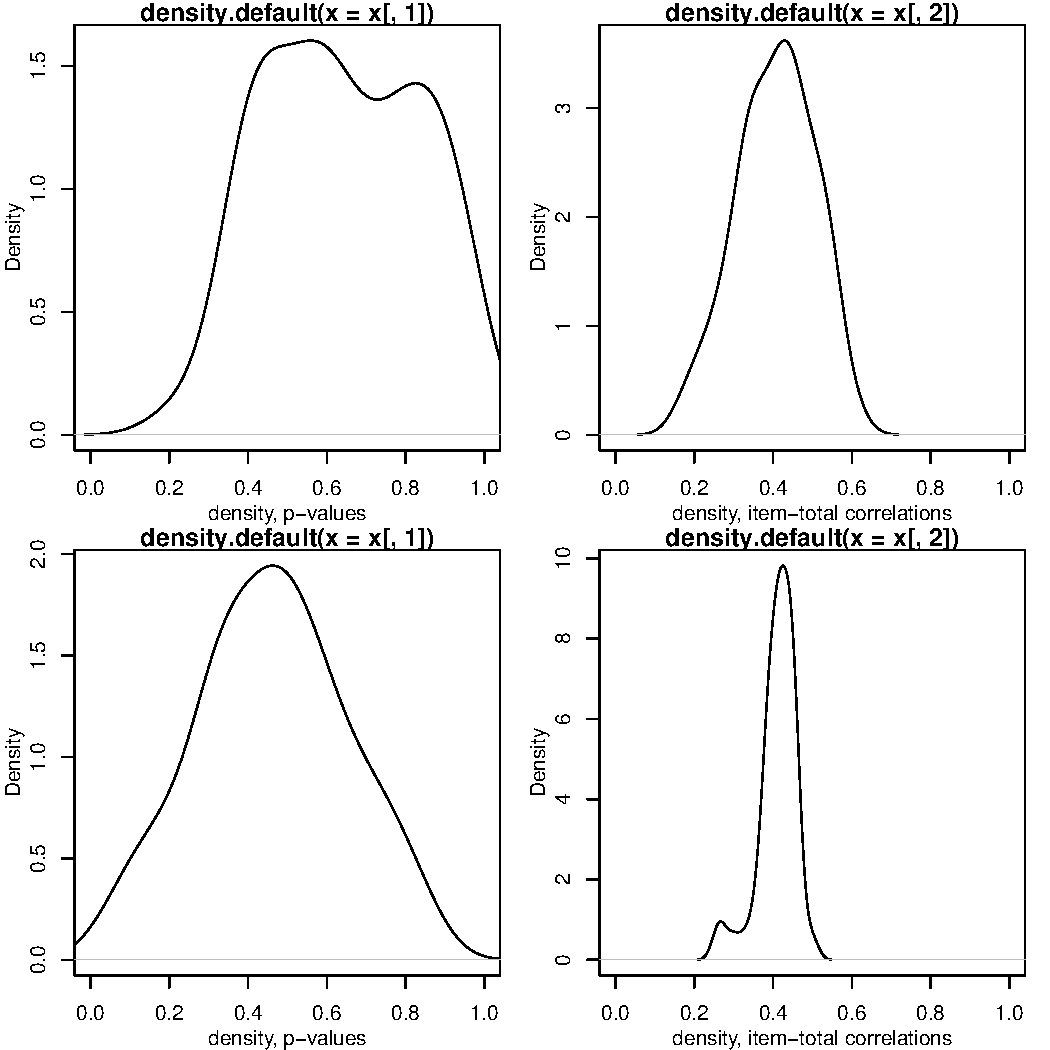
\includegraphics[width=\maxwidth]{figure/unnamed-chunk-13-2} 

\end{knitrout}


The simulated data set (bottom row of graphs) has a fairly normal distribution of item difficulty, while the empirical set (top row of graphs) essentially only consists of items that are middling difficulty or very easy.  When you look to the discrimination of the items (from the item-total correlation graphs), the simulated data set has a very consistently middling discrimination that is nearly the same for almost all items, while the empirical data set, once again, has a wider range of values, with a small number of more discriminating items and some items that are hardly discriminating at all. 


The interpretation, then, is that the empirical data set does not represent a ``good" instrument.  There are not a variety of item difficulties and the items themselves are not discriminating.

\pagebreak
\section{Buffon's Needle}

\begin{knitrout}
\definecolor{shadecolor}{rgb}{0.969, 0.969, 0.969}\color{fgcolor}\begin{kframe}
\begin{alltt}
\hlstd{n} \hlkwb{<-} \hlnum{1000} \hlcom{#number of needles}
\hlstd{d} \hlkwb{<-} \hlnum{1} \hlcom{#line spacing}
\hlstd{l} \hlkwb{<-} \hlnum{1} \hlcom{#needle length}

\hlcom{#matrix to hold all of the information about the needles}
\hlstd{orient} \hlkwb{<-} \hlkwd{matrix}\hlstd{(}\hlnum{NA}\hlstd{,n,}\hlnum{4}\hlstd{)}
\hlcom{#generates the position of the lefthand side of the needle}
\hlstd{orient[,}\hlnum{1}\hlstd{]} \hlkwb{<-} \hlkwd{runif}\hlstd{(n,}\hlnum{0}\hlstd{,d)}
\hlcom{#generates the angular orientation of the needle}
\hlstd{orient[,}\hlnum{2}\hlstd{]} \hlkwb{<-} \hlkwd{runif}\hlstd{(n,}\hlopt{-}\hlstd{pi}\hlopt{/}\hlnum{2}\hlstd{, pi}\hlopt{/}\hlnum{2}\hlstd{)}
\hlcom{#determines the horizontal span of the needle}
\hlstd{orient[,}\hlnum{3}\hlstd{]} \hlkwb{<-} \hlstd{orient[,}\hlnum{1}\hlstd{]}\hlopt{+}\hlstd{l}\hlopt{*}\hlkwd{cos}\hlstd{(orient[,}\hlnum{2}\hlstd{])}
\hlcom{#checks the location of the righthand side of the needle}
\hlstd{orient[,}\hlnum{4}\hlstd{]} \hlkwb{<-} \hlstd{orient[,}\hlnum{3}\hlstd{]} \hlopt{>=} \hlstd{d}
\hlcom{#determines the probability that a needle crossed a line}
\hlstd{p} \hlkwb{<-} \hlkwd{sum}\hlstd{(orient[,}\hlnum{4}\hlstd{])}\hlopt{/}\hlstd{n}
\hlstd{p}
\end{alltt}
\begin{verbatim}
## [1] 0.632
\end{verbatim}
\end{kframe}
\end{knitrout}

The approach I took here was based upon the following logic:
\begin{enumerate}
  \item This is a 1-dimensional problem.  The only thing that actually matters is the projection of the length of a particular needle onto a line perpendicular to the lines on the surface.
  \item It's only worth considering two lines, separated by a distance $d$.  
  \item Each needle lands with its leftmost edge some distance from that line on the left and makes some angle, $\theta$, with the line we are projecting its length onto.
  \item Since we always reference the leftmost edge of the needle, we only need to consider angles between $-\frac{\pi}{2}$ and $\frac{\pi}{2}$.
  \item If the distance between the leftmost edge and the line plus the projection of the length of the needle onto the perpendicular line is greater than the separation between the parallel lines, the needle will overlap a line.
\end{enumerate}
\end{document}
